\documentclass[a4paper,12pt]{article}

\tolerance=1
\emergencystretch=\maxdimen
\hyphenpenalty=10000
\hbadness=10000

\usepackage{fontspec}
\usepackage[T1]{fontenc}
\usepackage{lmodern}
\usepackage{makecell}
\usepackage{lmodern}
\usepackage{geometry}
\usepackage{longtable}
\usepackage{tabularx}
\usepackage{booktabs}
\geometry{left=2.5cm, right=2.5cm, top=2.5cm, bottom=5cm}
\usepackage{array}
\usepackage{xcolor}
\usepackage{graphicx}
\usepackage{titlesec}
\usepackage{xcolor}
\usepackage{fancyhdr}
\pagestyle{plain}
\setlength{\headheight}{67pt}   % height of the header box
\setlength{\headsep}{25pt}      % vertical space between header and body text
\setlength{\footskip}{30pt}     % distance from bottom of body to bottom of footer
\newcolumntype{C}[1]{>{\centering\let\newline\\\arraybackslash\hspace{0pt}}m{#1}}
\renewcommand{\headrulewidth}{0pt}
\renewcommand*{\thesection}{\Alph{section}}

\definecolor{darkblue}{RGB}{0,0,139}

\titleformat{\section}
  {\normalfont\Large\bfseries\color{darkblue}} % format
  {\thesection}{1em}{}                          % label + spacing

\titlespacing*{\section}
  {0pt}
  {0pt}
  {10pt}

\titlespacing*{\subsection}
  {0pt}
  {12pt}
  {8pt}

\titlespacing*{\subsubsection}
  {0pt}
  {12pt}
  {8pt}

\fancypagestyle{plain}{
  \fancyhf{}
  \fancyhead[]{
    \begin{center}
      \begin{tabular}{|C{10cm}|C{3.5cm}|}
        \hline
        \textbf{Corso di Ingegneria del Software} \newline Deliverable di progetto & \textbf{2024--2025} \\
        \hline
      \end{tabular}
    \end{center}
  }
  \fancyfoot[]{
    \begin{center}
      \begin{tabular}{|C{2cm}|C{11.5cm}|}
        \hline
        \thepage & \\
        \hline
      \end{tabular}

    \end{center}
  }

}
\fancypagestyle{title}{
  \fancyhf{}
  \fancyhead[C]{
    \begin{tabular}{|C{10cm}|C{3.5cm}|}
      \hline
      \textbf{Corso di Ingegneria del Software} \newline Deliverable di progetto & \textbf{2024--2025} \\
      \hline
    \end{tabular}
  }
  \renewcommand{\footrulewidth}{0pt}
}


\begin{document}

\begin{titlepage}
  \begin{center}
    \thispagestyle{title}
    \vspace*{1.5cm}

    \begin{center}
      {\LARGE \textbf{\textcolor{blue}{``Ingegneria del Software''}}}\\[0.3cm]
      {\LARGE \textbf{\textcolor{blue}{2024--2025}}}\\[1cm]
      {\normalsize \textbf{\textcolor{blue}{Docente: Prof. Angelo Furfaro}}}\\[1.2cm]
      {\Huge \textbf{\textcolor{red}{Gestore libreria}}}\\[0.3cm]
      {\Huge \textbf{\textcolor{red}{personale}}}
    \end{center}

    \vspace*{2.5cm}

    \noindent
    \begin{tabular}{|>{\bfseries}p{3cm}|p{12cm}|}
      \hline
      Data & <gg/mm/aaaa> \\
      Documento & Documento Finale -- D3 \\
      \hline
    \end{tabular}

    \vspace*{2.5cm}

    \begin{tabular}{|l|l|l|}
      \hline
      \multicolumn{3}{|c|}{\large \textbf{\textcolor{blue}{Team Members}}} \\
      \hline
      \textbf{Nome e Cognome} & \textbf{Matricola} & \textbf{E-mail address} \\
      \hline
      Leonardo Napoli & 234364 & npllrd02s30d086d@studenti.unical.it \\
      \hline
    \end{tabular}
  \end{center}
\end{titlepage}

\tableofcontents
\newpage
\pagestyle{plain}
{\Large \textbf{List of Challenging/Risky Requirements or Tasks}\label{list-of-challengingrisky-requirements-or-tasks}}

\begin{center}
  \begin{tabularx}{\textwidth}{|X|X|X|X|}
    \hline
    \textbf{Challenging Task}&
    \textbf{Date the task is identified}&
    \textbf{Date the challenge is resolved}&
    \textbf{Explanation on how the challenge has been managed}\\
    \hline
  \end{tabularx}
\end{center}

\newpage
\section{Stato dell'arte}

Tra le applicazioni maggiormente utilizzate per la gestione di librerie
ho potuto testare almeno 2 soluzioni utili. Si tratta di
Obsidian e Calibre.

\subsection{Obsidian}

Obsidian è un'applicazione più generalmente utilizzata per la creazione
di note, mappe mentali eappunti personali, ma grazie alla grande
possibilità che essa offre in termini di personalizzazione, si può
adattare a qualsiasi utilizzo. Uno dei tanti utilizzi da me provati è
stato proprio quello di mantenere la mia collezione di libri, con tanto
di immagine di copertina, valutazione e commenti.

\subsubsection{Vantaggi}

\begin{itemize}
  \item
    Personalizzazione praticamente illimitata grazie ai plugin
    open-source;
  \item
    Possibilità di creare collegamenti tra libri e/o commenti;
  \item
    Informazioni memorizzate in locale tramite file .md;
\end{itemize}

\subsubsection{Svantaggi}

\begin{itemize}
  \item
    La gestione di una libreria devia dallo scopo generale
    dell'applicazione;
  \item
    Complessa inizializzazione da parte di un utente non tecnico;
\end{itemize}

\subsection{Calibre}

Calibre è un'applicazione open-source orientata alla gestione di Ebook,
offre strumenti molto utili come la conversione di formati, gestione di
metadati e sincronizzazione tra dispositivi

\subsubsection{Vantaggi}

\begin{itemize}
  \item
    Software maturo ed open-source;
  \item
    Estendibile con plugin;
  \item
    Totalmente in locale;
\end{itemize}

\subsubsection{Svantaggi}

\begin{itemize}
  \item
    L'applicazione risulta inutile per la gestione di libri cartacei;
  \item
    Eccessive funzionalità offerte rendono l'interfaccia molto complessa.
\end{itemize}

\subsection{Considerazioni}

Osservando punti di forza e di debolezza delle applicazioni menzionate
si è potuto derivare alcune funzionalità utili che saranno implementate
nel sistema:

\begin{itemize}
  \item
    Salvataggio dei dati in locale ed esportabile;
  \item
    Gestione semplice tramite interfaccia grafica;
  \item
    Funzioni limitate per un approccio minimale;
  \item
    Possibilità di aggiunta di funzionalità aggiuntive.
\end{itemize}

\newpage
\section{Raffinamento dei Requisiti}
\subsection{Servizi (con prioritizzazione)}

\begin{enumerate}
  \item
    \textbf{Memorizzazione in memoria secondaria}. Importanza alta,
    complessità bassa. Tutti i dati immagazzinati nel sistema dovranno
    essere trasferiti in memoria secondaria quando salvati.
  \item
    \textbf{Creazione elementi}. Importanza alta, complessità bassa. Sarà
    possibile creare sia dei libri che delle collezioni di essi da
    gestire.
  \item
    \textbf{Lettura elementi.} Importanza alta, complessità bassa. Sarà
    possibile accedere ai dati dei libri e delle collezioni memorizzate.
  \item
    \textbf{Modifica elementi.} Importanza alta, complessità bassa. Sarà
    possibile modificare i dati relativi agli elementi memorizzati.
  \item
    \textbf{Rimozione elementi.} Importanza alta, complessità bassa. Sarà
    possibile rimuovere elementi mantenendo il sistema in uno stato
    accettabile.
  \item
    \textbf{Cambiamento stato libro.} Importanza alta, complessità bassa.
    Ogni libro avrà tra i suoi attributi lo stato di lettura, che potrà
    essere ``letto'', ``da leggere'', ``in lettura''.
  \item
    \textbf{Ricerca e ordinamento.} Importanza alta, complessità media.
    Ogni dato presente potrà essere ricercato e ordinato secondo i criteri
    disponibili.
  \item
    \textbf{Virtualizzazione libreria.} Importanza media, complessità
    media. Il sistema formerà una libreria virtuale corrispondente a
    quella fisica, così da velocizzare la ricerca dei volumi.
  \item
    \textbf{Interfaccia grafica.} Importanza alta, complessità alta. Il
    sistema con le sue funzionalità potrà essere interamente utilizzato
    tramite interfaccia grafica.
\end{enumerate}

\subsection{Requisiti non Funzionali}

\begin{itemize}
  \item
    \textbf{Multithreading.} Il sistema dovrà poter essere utilizzato in
    multithreading in maniera sicura.
  \item
    \textbf{Consistenza dei dati.} I dati inseriti dovranno rimanere
    consistenti a fronte di qualsiasi operazione messa a disposizione dal
    sistema.
  \item
    \textbf{Manutenibilità.} Il sistema deve essere ben strutturato così
    da garantire aggiornamenti ed aggiunta di funzionalità.
  \item
    \textbf{Portabilità.} Il sistema deve essere utilizzabile sugli OS più
    comuni, quindi Linux, MacOs e Windows.
\end{itemize}

\subsection{Scenari d'uso dettagliati con relativi Use Case
Diagrams}

\subsubsection{Aggiunta libro}\label{aggiunta-libro}

\begin{itemize}
  \item
    L'utente preme sul tasto ``Aggiungi libro'';
  \item
    L'utente inserisce le informazioni: titolo, autore, ISBN, genere;
  \item
    L'utente conferma le informazioni;
  \item
    L'utente preme sul tasto ``Salva''.
\end{itemize}

\begin{center}
  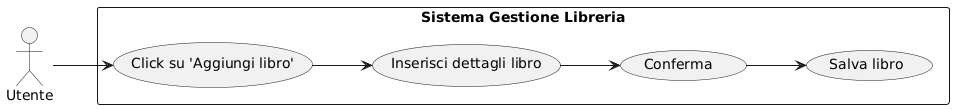
\includegraphics[width = \textwidth]{media/useCase1.png}
\end{center}

\subsubsection{Aggiunta collezione}\label{aggiunta-collezione}

\begin{itemize}
  \item
    L'utente preme sul tasto ``Aggiungi collezione'';
  \item
    L'utente inserisce il nome della collezione;
  \item
    L'utente \underline{ricerca l'elemento desiderato;}
  \item
    L'utente preme il tasto ``Aggiungi'';
  \item
    L'utente ripete le ultime 3 operazioni quante volte desidera;
  \item
    L'utente conferma le informazioni;
  \item
    L'utente preme sul tasto salva.
\end{itemize}

\begin{center}
  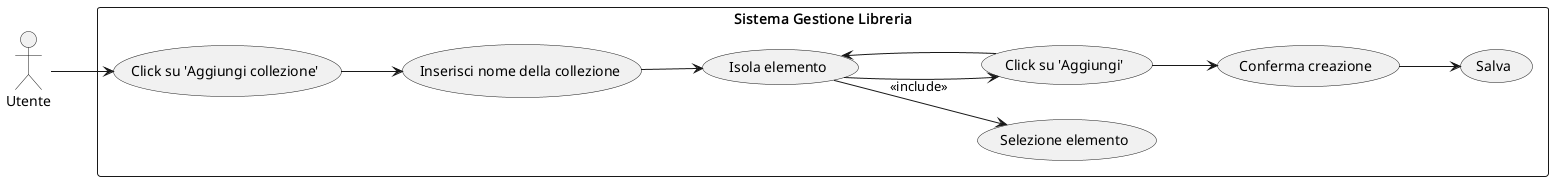
\includegraphics[width=5.10903in,height=0.70625in]{media/useCase2.png}
\end{center}

\subsubsection{Selezione elemento}\label{selezione-elemento}

\begin{itemize}
  \item
    L'utente digita parola chiave nell'apposita casella;
  \item
    L'utente clicca su ``Ricerca'';
  \item
    Il sistema restituisce una lista di risultati;
  \item
    L'utente clicca sul risultato desiderato;
\end{itemize}

\begin{center}
  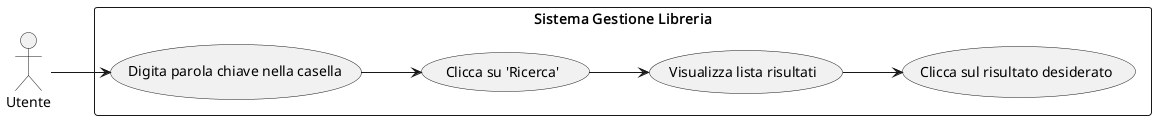
\includegraphics[width=\textwidth]{media/useCase3.png}
\end{center}

\subsubsection{Modifica dati}\label{modifica-dati}

\begin{itemize}
  \item
    L'utente \underline{ricerca l'elemento desiderato;}
  \item
    L'utente preme sul tasto ``Modifica'';
  \item
    L'utente preme spunta la casella del campo che desidera modificare;
  \item
    L'utente digita il nuovo valore dell'attributo;
  \item
    L'utente preme su ``Termina modifica'';
  \item
    L'utente visualizza un'anteprima dell'elemento modificato;
  \item
    L'utente preme il tasto ``Conferma''.
\end{itemize}

\begin{center}
  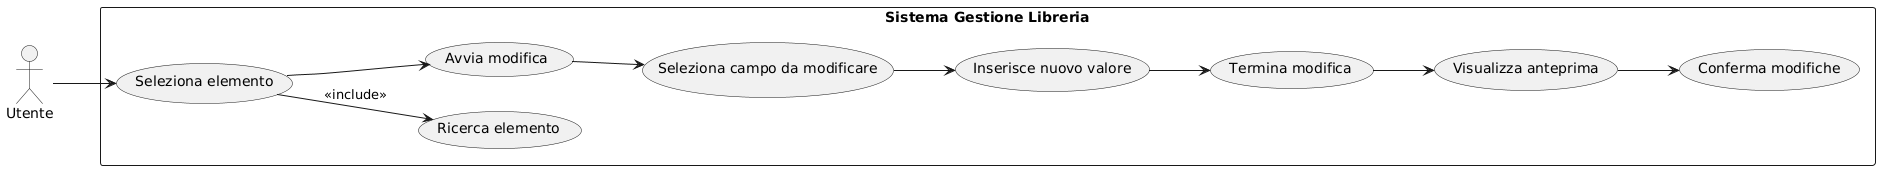
\includegraphics[width=\textwidth]{media/useCase4.png}
\end{center}

\subsubsection{Elimina elemento}\label{elimina-elemento}

\begin{itemize}
  \item
    L'utente \underline{ricerca l'elemento desiderato}
  \item
    L`utente preme il tasto su 'Elimina';
  \item
    L'utente preme il tasto 'Conferma';
\end{itemize}
\begin{center}
  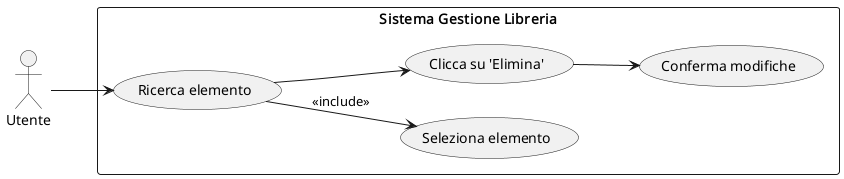
\includegraphics[width=\textwidth]{media/useCase5.png}
\end{center}

\subsubsection{Avanza stato libro}
\begin{itemize}
  \item
    L'utente \underline{ricerca un libro};
  \item
    L`utente preme il tasto utile all'avanzamento della lettura;
\end{itemize}
\begin{center}
  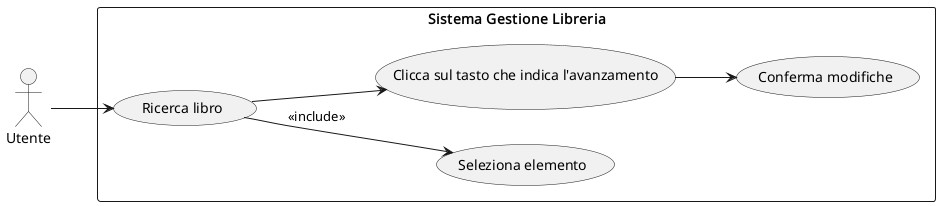
\includegraphics[width=\textwidth]{media/useCase6.png}
\end{center}

\subsection{Funzionalità escluse}

\begin{itemize}
  \item
    \textbf{Sincronizzazione su più dispositivi}, non rientra nella filosofia dell'applicazione, che si pone come una libreria completamente offline.
  \item
    \textbf{Gestione di segnalibri}, sarebbero funzioni più legate alla gestione di ebook, che non è l'obiettivo della nostra applicazione.
  \item
    \textbf{Recupero automatico di metadati}, comprometterebbe il funzionamento in locale.
\end{itemize}

\subsection{Assunzioni}
\emph{\textless Briefly document, in this section, the most relevant
  requirement assumptions/decisions you had to made during your
project\textgreater{}}
\begin{itemize}
  \item L'applicazione sarà monoutente. Questa decisione rientra nella filosofia per la quale l'applicazione nella sua interezza si pone come una libreria virtuale.
  \item Tutti i dati saranno in locale, con possibilità di esportarli in file di più formati.
  \item Le modifiche saranno prima salvate in memoria principale, per poi essere trasferite in memoria secondaria soltanto al momento del salvataggio. Questa decisione é stata presa per migliorare le prestazioni.
  
\end{itemize}

\newpage
\section{Architettura Software}
\emph{\textless IF RELEVANT, Report here both the static and the dynamic
  view of your system design, in terms of a Component Diagram, and their
related Sequence Diagrams \textgreater{}}

\subsection{The static view of the system: Component Diagram}

\subsection{The dynamic view of the software architecture:
Sequence Diagram}

\newpage
\section{Dati e la loro modellazione}

\emph{Definite le sorgenti di dati a voi necessarie per realizzare I
  servizi di cui sopra. Modellate tali dati tramite un ER o similari.
  Specificate se e quali di tali dati sono gia' forniti da applicativi
esistenti.}

\newpage
\section{Scelte Progettuali (Design Decisions)}
\textless Document here the \textbf{5} most important design decisions
you had to take. You can use both a textual or a diagrammatic
specification.\textgreater{}

\newpage
\section{Progettazione di Basso Livello}

\newpage
\section{Spiegare come il progetto soddisfa i requisiti funzionali (FRs) e
quelli non funzionali (NFRs)}
\emph{\textless Report in this section how
  the architectural and low level design you produced satisfies the FRs
and the NFRs\textgreater{}}

Appendix. Prototype\\
\emph{\textless Provide
  a brief report on your prototype, and especially: information on what
  you have implemented, how the implementation covers the FR and NFR, how
  the prototypes demonstrates your project correctness with respect to the
  FR and NFR. You may add some screenshots to describe what required
  above. Be ready to show your prototype during the oral
examination\textgreater{}}
\end{document}
